\documentclass[12pt,a4paper]{article}
\usepackage[utf8]{inputenc}
\usepackage{amsmath}
\usepackage{amssymb}
\usepackage{amsthm}
\usepackage{geometry}
\usepackage{tikz}
\usetikzlibrary{trees, calc, positioning}

% Page layout
\geometry{margin=1in}

% Theorem environments
\theoremstyle{definition}
\newtheorem{problem}{Problem}
\newtheorem{solution}{Solution}

\title{\textbf{Rigorous Resolution Refutation and Construction}}
\author{}
\date{}

\begin{document}

\maketitle

\section*{Part (a): Resolution Refutation Tree}

\begin{problem}
Let $\varphi$ be the CNF formula defined by the following set of clauses:
\begin{align*}
    C_1 &= (x_1 \lor x_2 \lor x_3 \lor x_4) \\
    C_2 &= (\neg x_1 \lor x_2 \lor x_4) \\
    C_3 &= (x_1 \lor \neg x_2 \lor \neg x_3) \\
    C_4 &= (\neg x_2 \lor x_3) \\
    C_5 &= (x_2 \lor \neg x_3) \\
    C_6 &= (\neg x_4 \lor x_3) \\
    C_7 &= (\neg x_1 \lor \neg x_3)
\end{align*}
Show that $\varphi$ is unsatisfiable using only the resolution rule.
\end{problem}

\begin{solution}
We perform a proof by resolution refutation. We aim to derive the empty clause ($\square$) by resolving pairs of clauses containing complementary literals.

\subsection*{Step-by-Step Derivation}

\textbf{Step 1: Eliminate variable $x_4$} \\
Resolve $C_1$ with $C_6$ on $x_4$:
$$ \frac{(x_1 \lor x_2 \lor x_3 \lor x_4) \quad (\neg x_4 \lor x_3)}{(x_1 \lor x_2 \lor x_3)} \quad \text{(Label } R_1 \text{)} $$
Resolve $C_2$ with $C_6$ on $x_4$:
$$ \frac{(\neg x_1 \lor x_2 \lor x_4) \quad (\neg x_4 \lor x_3)}{(\neg x_1 \lor x_2 \lor x_3)} \quad \text{(Label } R_2 \text{)} $$

\textbf{Step 2: Eliminate variable $x_1$} \\
Resolve $R_1$ with $R_2$ on $x_1$:
$$ \frac{(x_1 \lor x_2 \lor x_3) \quad (\neg x_1 \lor x_2 \lor x_3)}{(x_2 \lor x_3)} \quad \text{(Label } R_3 \text{)} $$
Resolve $C_3$ with $C_7$ on $x_1$:
$$ \frac{(x_1 \lor \neg x_2 \lor \neg x_3) \quad (\neg x_1 \lor \neg x_3)}{(\neg x_2 \lor \neg x_3)} \quad \text{(Label } R_4 \text{)} $$

\textbf{Step 3: Eliminate variable $x_2$} \\
Resolve $R_3$ with $C_4$ on $x_2$:
$$ \frac{(x_2 \lor x_3) \quad (\neg x_2 \lor x_3)}{(x_3)} \quad \text{(Label } R_5 \text{)} $$
Resolve $R_4$ with $C_5$ on $x_2$:
$$ \frac{(\neg x_2 \lor \neg x_3) \quad (x_2 \lor \neg x_3)}{(\neg x_3)} \quad \text{(Label } R_6 \text{)} $$

\textbf{Step 4: Derive Empty Clause} \\
Resolve the unit clauses $R_5$ and $R_6$ on $x_3$:
$$ \frac{(x_3) \quad (\neg x_3)}{\square} $$

Since we have derived the empty clause, the original formula $\varphi$ is unsatisfiable.

\subsection*{Resolution Refutation Tree}

\begin{center}
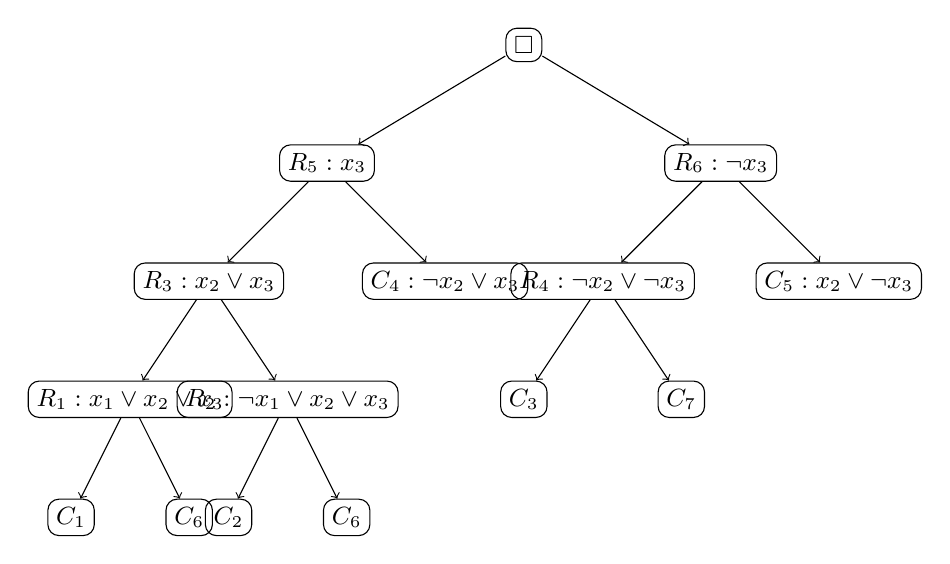
\begin{tikzpicture}[
    level 1/.style={sibling distance=50mm},
    level 2/.style={sibling distance=30mm},
    level 3/.style={sibling distance=20mm},
    level 4/.style={sibling distance=15mm},
    every node/.style={draw, rectangle, rounded corners, align=center, inner sep=3pt, font=\small},
    edge from parent/.style={draw, ->}
]

\node {$\square$}
    child { node {$R_5: x_3$}
        child { node {$R_3: x_2 \lor x_3$}
            child { node {$R_1: x_1 \lor x_2 \lor x_3$}
                child { node {$C_1$} }
                child { node {$C_6$} }
            }
            child { node {$R_2: \neg x_1 \lor x_2 \lor x_3$}
                child { node {$C_2$} }
                child { node {$C_6$} }
            }
        }
        child { node {$C_4: \neg x_2 \lor x_3$} }
    }
    child { node {$R_6: \neg x_3$}
        child { node {$R_4: \neg x_2 \lor \neg x_3$}
            child { node {$C_3$} }
            child { node {$C_7$} }
        }
        child { node {$C_5: x_2 \lor \neg x_3$} }
    };

\end{tikzpicture}
\end{center}

\end{solution}

\newpage

\section*{Part (b): Construction of Unsatisfiable Formula $\beta$}

\begin{problem}
Let $\alpha$ be an \textit{unsatisfiable} CNF formula with $m$ clauses over $n$ variables, where the minimum number of literals in a clause is $r$ ($m, n \ge 1, r \ge 2$). Show that there exists a CNF formula $\beta$ such that:
\begin{itemize}
    \item $\beta$ is unsatisfiable.
    \item $\beta$ has $m+1$ clauses and $n+1$ variables.
    \item $\alpha$ and $\beta$ share $m-1$ clauses.
    \item The minimum number of literals in a clause of $\beta$ is $r$.
\end{itemize}
\end{problem}

\begin{solution}
Let the clause set of $\alpha$ be $\{C_1, C_2, \dots, C_m\}$ over the variable set $X = \{x_1, \dots, x_n\}$.
Since $\alpha$ is unsatisfiable, the conjunction $\bigwedge_{i=1}^m C_i$ evaluates to False for all truth assignments to $X$.

\subsubsection*{Construction of $\beta$}
We introduce a new variable $x_{n+1} \notin X$.
We select the last clause of $\alpha$, denoted $C_m$, and "split" it using the new variable.
We define $\beta$ as the conjunction of the first $m-1$ clauses of $\alpha$, plus two new clauses derived from $C_m$:
$$ \beta = \left( \bigwedge_{i=1}^{m-1} C_i \right) \land (C_m \lor x_{n+1}) \land (C_m \lor \neg x_{n+1}) $$

The set of clauses for $\beta$ is:
$$ S_\beta = \{C_1, C_2, \dots, C_{m-1}, D_1, D_2\} $$
where $D_1 = (C_m \lor x_{n+1})$ and $D_2 = (C_m \lor \neg x_{n+1})$.

\subsubsection*{Verification of Properties}

\textbf{1. $\beta$ is unsatisfiable:} \\
Suppose for contradiction that $\beta$ is satisfiable. Then there exists a truth assignment $V$ to variables $\{x_1, \dots, x_{n+1}\}$ such that all clauses in $S_\beta$ are true.
Specifically, $V$ must satisfy $D_1$ and $D_2$.
\begin{itemize}
    \item If $V(x_{n+1}) = \text{False}$, then $D_1 = (C_m \lor \text{False}) \equiv C_m$ must be true.
    \item If $V(x_{n+1}) = \text{True}$, then $D_2 = (C_m \lor \text{False}) \equiv C_m$ must be true.
\end{itemize}
In either case, $V$ must satisfy $C_m$. Since $V$ also satisfies $\{C_1, \dots, C_{m-1}\}$, $V$ satisfies all clauses of $\alpha$. This contradicts the premise that $\alpha$ is unsatisfiable. Thus, $\beta$ is unsatisfiable.

\textbf{2. $\beta$ has $m+1$ clauses and $n+1$ variables:} \\
\begin{itemize}
    \item \textbf{Clauses:} $\beta$ contains the first $m-1$ clauses of $\alpha$ and the 2 new clauses $D_1, D_2$. Total clauses $= (m-1) + 2 = m+1$.
    \item \textbf{Variables:} $\beta$ is defined over $X \cup \{x_{n+1}\}$. Total variables $= n + 1$.
\end{itemize}

\textbf{3. $\alpha$ and $\beta$ share $m-1$ clauses:} \\
The intersection of the clause sets is $\{C_1, \dots, C_{m-1}\}$. The size of this set is exactly $m-1$.

\textbf{4. Minimum number of literals is $r$:} \\
Let $|C|$ denote the number of literals in clause $C$. We are given that $\min_{C \in \alpha} |C| = r$.
\begin{itemize}
    \item For the shared clauses $C_i$ ($1 \le i \le m-1$), $|C_i| \ge r$.
    \item For the new clauses $D_1$ and $D_2$, $|D_1| = |D_2| = |C_m| + 1$.
    \item Since $|C_m| \ge r$, we have $|D_1| = |D_2| \ge r+1$.
\end{itemize}
The minimum length in $\beta$ is $\min( \min_{i<m} |C_i|, |C_m|+1 )$. Since all $|C_i| \ge r$, the minimum remains $r$.

\end{solution}

\end{document}